\documentclass[a4paper,11pt]{article}
\usepackage{graphicx}
\usepackage{enumerate}
\usepackage[usenames, dvipsnames]{color}

\begin{document}

\begin{flushright}

\vspace{1.1cm}

{\bf\Huge Project 1}

\rule{0.25\linewidth}{0.5pt}

\vspace{0.5cm}
%Put Authors
Justin Ely
\linebreak
\newline
%Put Author's affiliations
\footnotesize{605.462 Data Visualization \\}
\vspace{0.5cm}
% Date here below
07 February, 2017
\end{flushright}

\noindent\rule{\linewidth}{1.0pt}

%%%%%%%%%%%%%%%%%%%%%%%%%%%%%%%%%%%%%%%%%%%%%%%%%%%%%%%%%%

\section{Pairing Wine and Food}
The visualization chosen, and shown in Figure 1, is a chart showing which types of wine best pair with various types of food.  Since the underlying data is not given in the website, so we assume it's simply the subjective feelings of the author.  As such, this commentary can't comment on the visualization's ability to represent the truth, but will focus on the clarity and effectiveness of the communication.  

\begin{figure}[h!]
\caption{Food and wine pairing map as compiled by winefolly.com.  Source: http://winefolly.com/review/5-tips-to-perfect-food-and-wine-pairing/} 
\centering
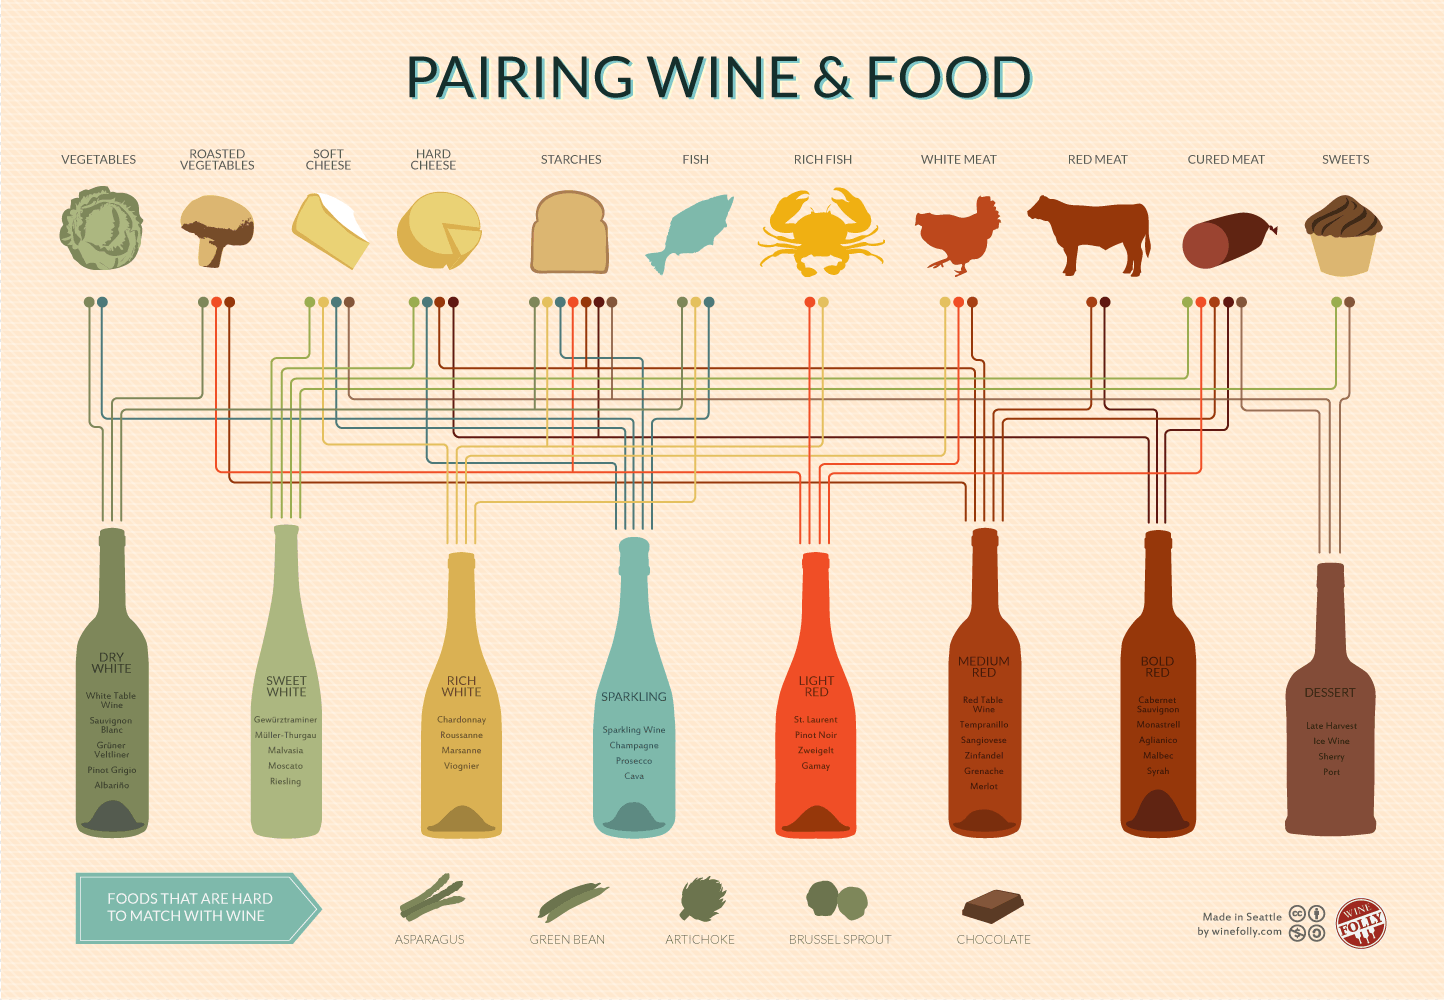
\includegraphics[width=1.1\textwidth]{wine-and-food-pairing-chart.png}
\end{figure}

\section{Type of Visualization}
This is a graph-type of visualization, where types of wine and food categories are nodes and each mapping is an edge.  The nodes are arranged in two parallel rows, with food on the top and wine on the bottom.  In addition, the types of wines and the food categories are also represented both by pictures and text.

\section{Effective}
The most effective part of this graphic are the pictures of the food.  Though it's moderately redundant with the text, its also an effective tool when this chart is used with just a quick glance.  Rather than having to read individual words, the eye can quickly jump to the meat, vegetables, etc very quickly.  

\section{Misleading}
This chart is more confusing than it is misleading, and most of the confusion comes from the connections between the wine and food.  There are too many lines mashed too closely together for the eye to easily follow.  There is an attempt to alleviate this with color, matched to the wine bottles, but the color progression chosen adds confusion as much as it helps.  The color-coding scheme of the wine bottles seems to almost have a consistent theme, but with just enough departures from commonality to confuse things.  Light-red through dessert wines, each increasing in shade, makes sense with a mental perception of growing richness.  However, the other end of the spectrum makes little sense.  Sparkling wine is a blue color, and the progressing whites change from a golden to a deep green.  

One might think the colors map closely to the colors of the food on the top axis, but this doesn't hold up for many of the mappings.  For example, the sweet white (a pale green) doesn't map to a single vegetable.  The sparkling (blue) does map to the blue fish, but also maps to starches, both cheeses, and the vegetables.

In addition to color, the chart lines seems to point in the wrong direction.  The line terminated in a dot draws the eye from the bottom to the top, making the viewer use the chart in a wine to food direction.  This is opposite of typical usage, where someone would have a meal and need to find wine to pair with it.  

\section{Improvements}
The simplest and best improvement I would make to this mapping would be to make it interactive.  As someone selects either a bottle or a food, anything it doesn't link to would fade into the background.  This would make the paths between the bottles stand out vividly, and avoid so much of the confusion and slowness when tracing paths.

Alternatively, if the chart must remain static, the wine bottles should be spread both above and below the food.  With the bottles more spread out, the criss-crossing lines will go down significantly and allow the paths to be more quickly traced.  

In either case, the colormaps should be adjusted.  Since there's no consistent mapping between wine and food, this should be dropped and each axis should be allowed to take on a self-consistent progression.  Additionally, the colors need to be chosen to be more colorblind friendly.  Even to my very slight color-blindness, the pale greens and reds are difficult to distinguish when the paths are densely packed.  This would help not only making the graphic more accessible to the public, but also preserve the information in a black and white print.

%%%%%%%%%%%%%%%%%%%%%%%%%%%%%%%%%%%%%%%%%%%%%%%%%%%%%%%%%%


\end{document}
